\section{Managing Cities}\label{sec:managing-cities}
The first functionality available to the user is to manage cities on the map. Several maps are available for selection, which are later, during the
visualization of the cube, cropped to the portion containing only cities relevant to the selected artists. This feature is important as it
dynamically changes the map to our needs, so the whole map with irrelevant locations is not included in the cube. Cities are added with a click on
the map using a small zoom-in lens, and their names and positions can be edited or deleted as well. During the addition of cities, their names are
entered in a modal dialog.

More information about how the map is cropped according to the artists’ residences, and the related parts of the project code, can be found in
\Cref{subsec:map-cropping}.

\begin{figure}[hbt!]
    \begin{center}
        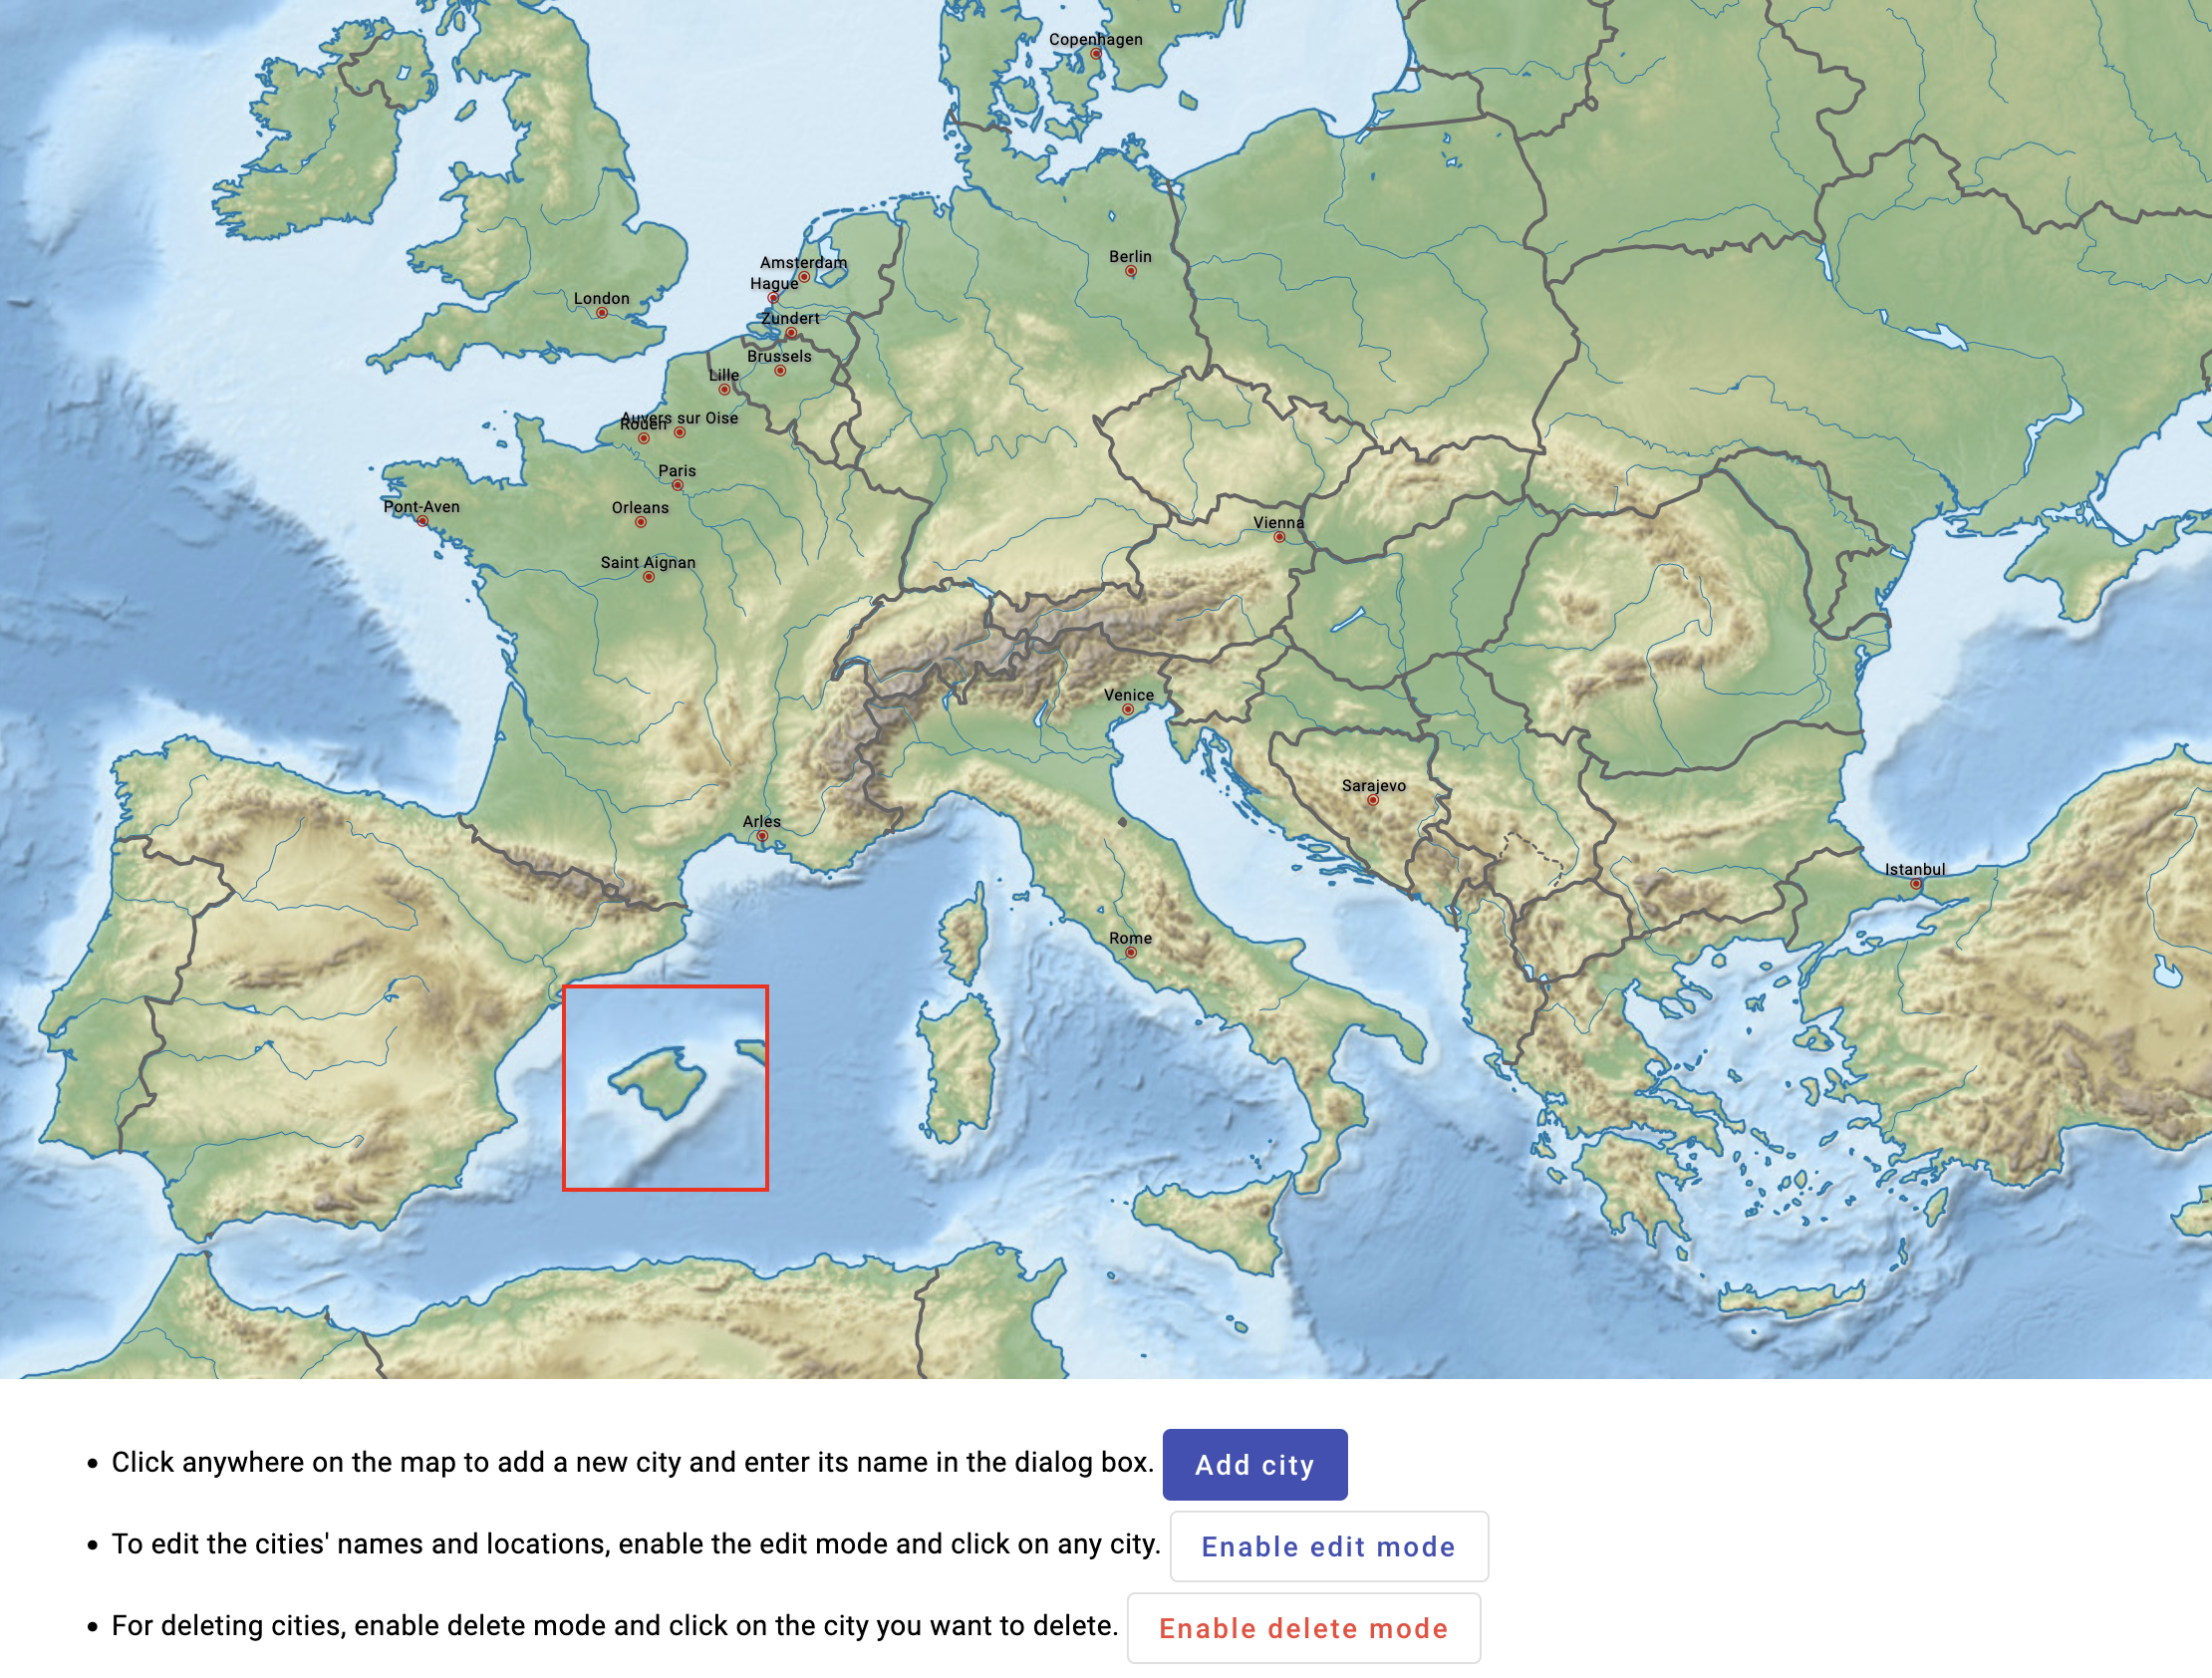
\includegraphics[width=\textwidth]{graphics/3-implementation/2}
    \end{center}
    \caption{Manage cities functionality page}
    \label{fig:figure3.2}
\end{figure}

\clearpage